\section{Диаграммы IDEF3}
\subsection{PFDD диаграммы}

\subsubsection{Контекстная диаграмма верхнего уровня}

Студенты и преподаватели взаимодействуют с системой,в результате чего на выходе
образуются проверенные тесты и удовлетворение потребностей преподавателей.

\begin{figure}[H]
    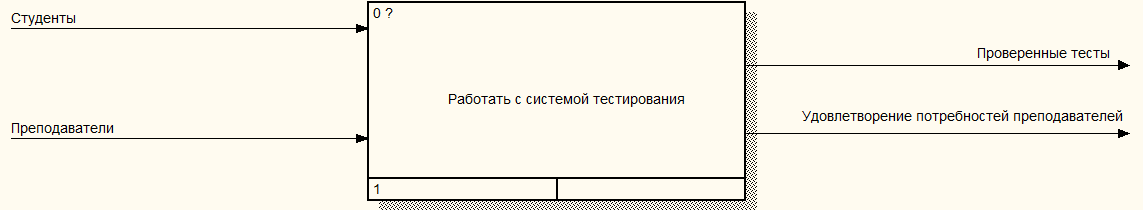
\includegraphics[width=\textwidth, center]{../img/idef3/Context.png}
    \caption{Контекстная диаграмма верхнего уровня}
\end{figure}

Данная диаграмма отображает наиболее общий вид модели системы тестирования.

\subsubsection{Работать с системой тестирования}
\begin{figure}[H]
    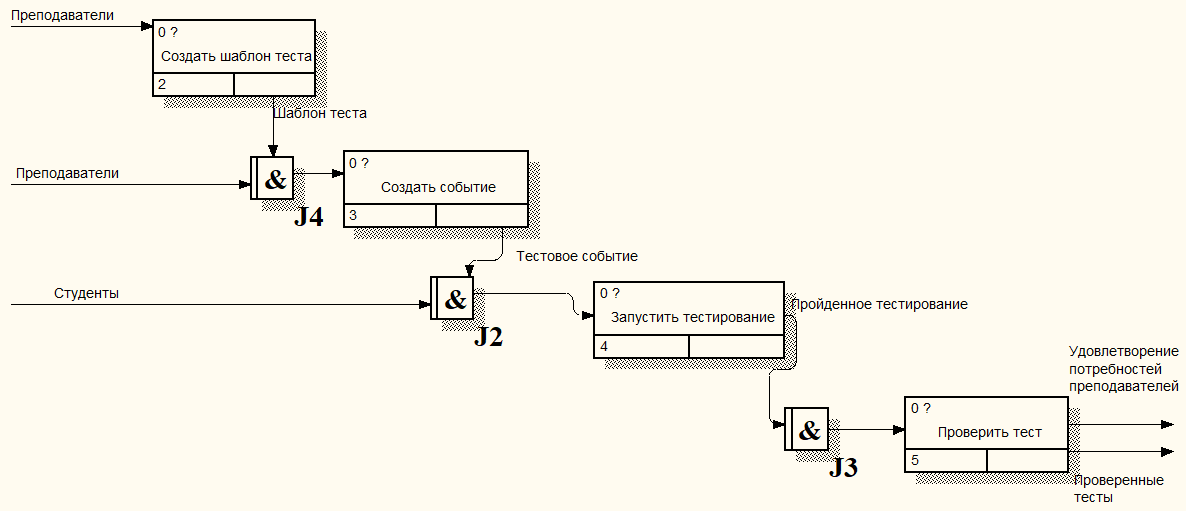
\includegraphics[width=\textwidth, center]{../img/idef3/ContextDecompose.png}
    \caption{Работать с системой тестирования}
\end{figure}

Преподаватели сначала создают шаблон теста, потом создают на основе этого шаблона
тестовое событие, которое запускают и проходят студенты, после чего пройденное 
тестирование проверяется системой на корректность, и результат проверки становится
доступен для студента, прошедшего тестирование и преподавателей.

\subsubsection{Создать шаблон теста}
\begin{figure}[H]
    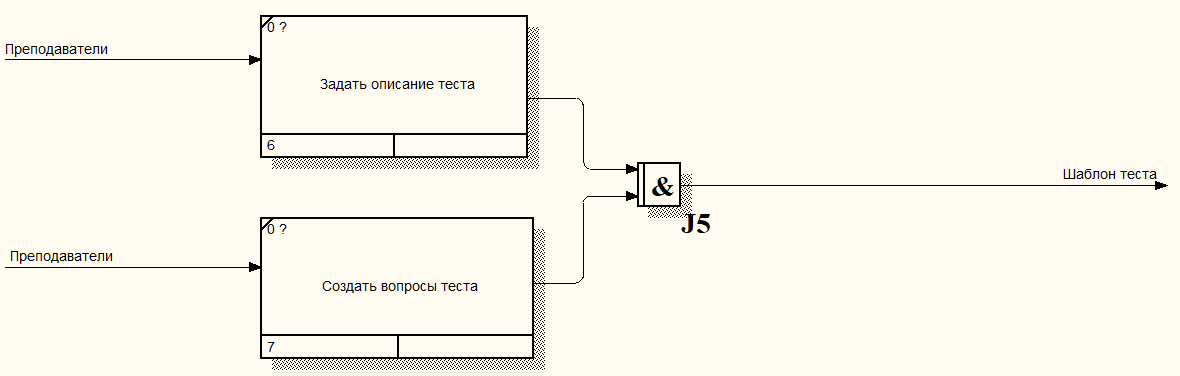
\includegraphics[width=\textwidth, center]{../img/idef3/CreateTestTemplate.png}
    \caption{Создать шаблон теста}
\end{figure}

Преподаватели задают описание теста и формируют вопросы теста, в результате чего
получает шаблон теста.

\subsubsection{Создать событие}
\begin{figure}[H]
    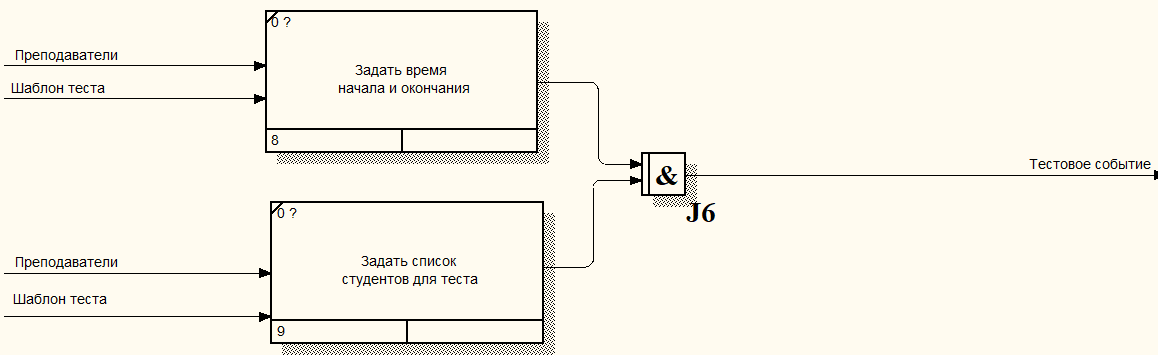
\includegraphics[width=\textwidth, center]{../img/idef3/CreateTestInstance.png}
    \caption{Создать событие}
\end{figure}

На основе шаблона теста преподаватель создает тестовое событие, для которого указывает
время начала и окончания и список студентов, которым необходимо принять участие
в этом событии.

\subsubsection{Запустить тестирование}
\begin{figure}[H]
    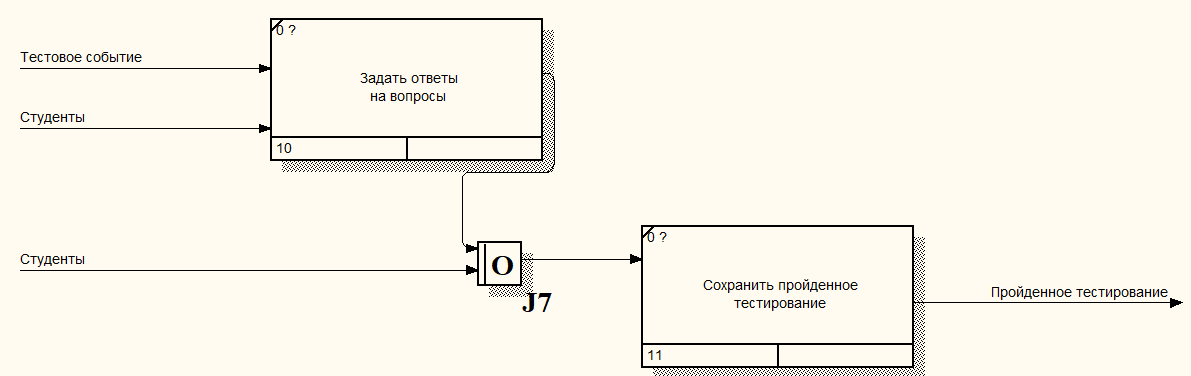
\includegraphics[width=\textwidth, center]{../img/idef3/RunTest.png}
    \caption{Запустить тестирование}
\end{figure}

Студент запускает выбранное тестовое событие и отвечает на вопросы теста,
если знает на них ответы. По завершении тестирования все ответы студента сохраняются.

\subsubsection{Проверить тестирование}
\begin{figure}[H]
    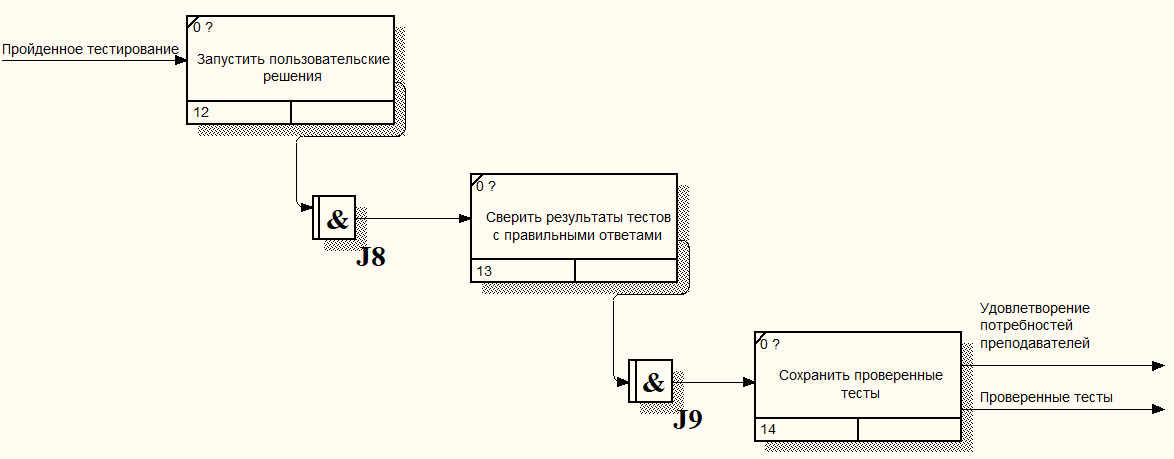
\includegraphics[width=\textwidth, center]{../img/idef3/ValidateTest.png}
    \caption{Проверить тестирование}
\end{figure}

После завершения тестирования система запускает код решений студента, получает
результаты работы алгоритмов и сравнивает их с правильными ответами на соответствующие вопросы.
После проверки результаты сохраняются и становятся доступны преподавателям и студенту,
проходившему тестирование.

\subsection{OSTN диаграмма}
\begin{figure}[H]
    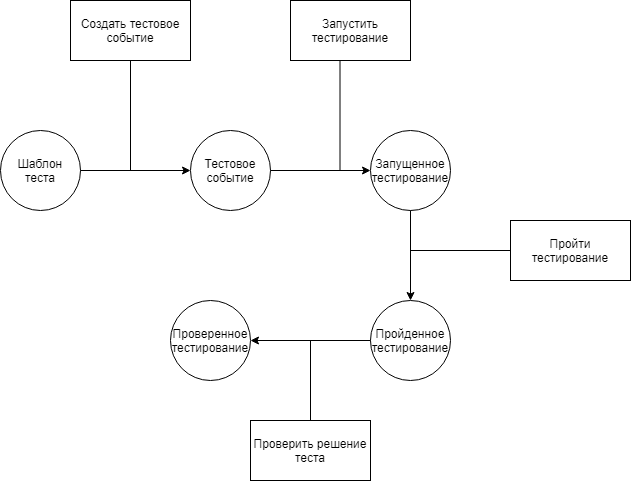
\includegraphics[width=\textwidth, center]{../img/OSTN.png}
    \caption{OSTN диаграмма}
\end{figure}

В системе не существует какого-то одного объекта, который подвергается изменениям.
Поэтому на данной диаграмме отображены основные объекты, которые присутствуют в
системе и образуются на различных этапах взаимодействия с ней.

Существуют следующие объекты:
\begin{enumerate}
    \item Шаблон теста
    \item Тестовое событие
    \item Запущенное тестирование
    \item Пройденное тестирование
    \item Проверенное тестирование
\end{enumerate}

Переходы:
\begin{enumerate}
    \item Шаблон теста -> Тестовое событие (событие создается на основе шаблона
    и имеет список назначенных на него студентов)
    \item Тестовое событие -> Запущенное тестирование (назначенный на событие студент
    может запустить его и начать проходить тестирование)
    \item Запущенное тестирование -> Пройденное тестирование (когда студент заканчивает
    прохождение тестирования, то оно становится пройденным, и его результаты сохраняются)
    \item Пройденное тестирование -> Проверенное тестирование (После прохождение тестирования
    система проверяет его и сохраняет результаты проверки)
\end{enumerate}


\subsection{DFD диаграммы}